\begin{frame}
	\frametitle{Encoding Parameters}
	
	\large{Number of Combinations}
	\begin{itemize}
		\item 6 source videos
		\item 3 resolutions \textendash\ 540p, 1080p, 2160p
		\item 3 average bitrates per resolution
		\item 2 encoding presets
	\end{itemize}
	108 final sequences
\end{frame}

\begin{frame}
	\frametitle{Encoding Parameters}
	
	\large{Encoding Presets}
	\begin{itemize}
		\item 2 different setting combinations for x265
		\item "na\"{\i}ve" preset \textendash\ CBR
		\item "expert" preset \textendash\ 2-pass encoding
	\end{itemize}
\end{frame}

\begin{frame}
	\frametitle{Encoding Parameters}
	\large{Selection of bitrates}
	\begin{itemize}
		\item Selection based on predicted encoding quality
		\item Using \textit{Video Multi-Method Assessment Fusion} (VMAF) \cite{lin2013:mmf}
		\item Scores computed at 25 bitrates per sequence with CBR
	\end{itemize}
\end{frame}

\begin{frame}
	\frametitle{Encoding Parameters}
	\begin{figure}
		\centering
		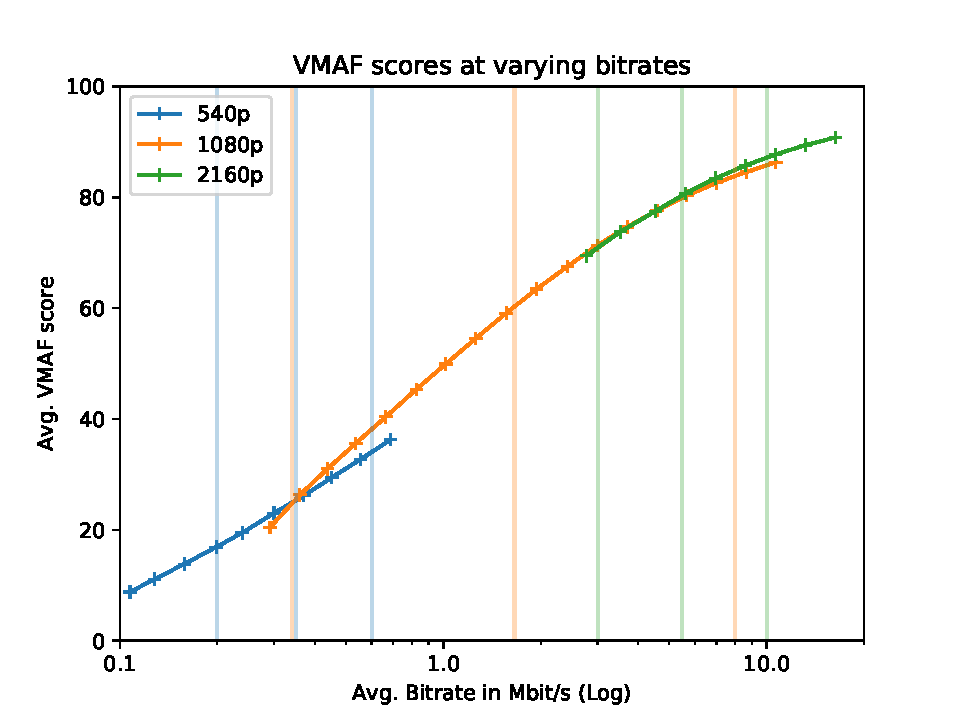
\includegraphics[width=2.8in]{vmaf_bitrates}
	\end{figure}
	Average \textit{VMAF} scores for 25 different bitrates at 3 resolutions.\\
	The vertical lines represent the selected bitrates.
\end{frame}

\begin{frame}
	\frametitle{Encoding Parameters}
	
	\large{Automated processing and encoding workflow.}

	\begin{figure}
		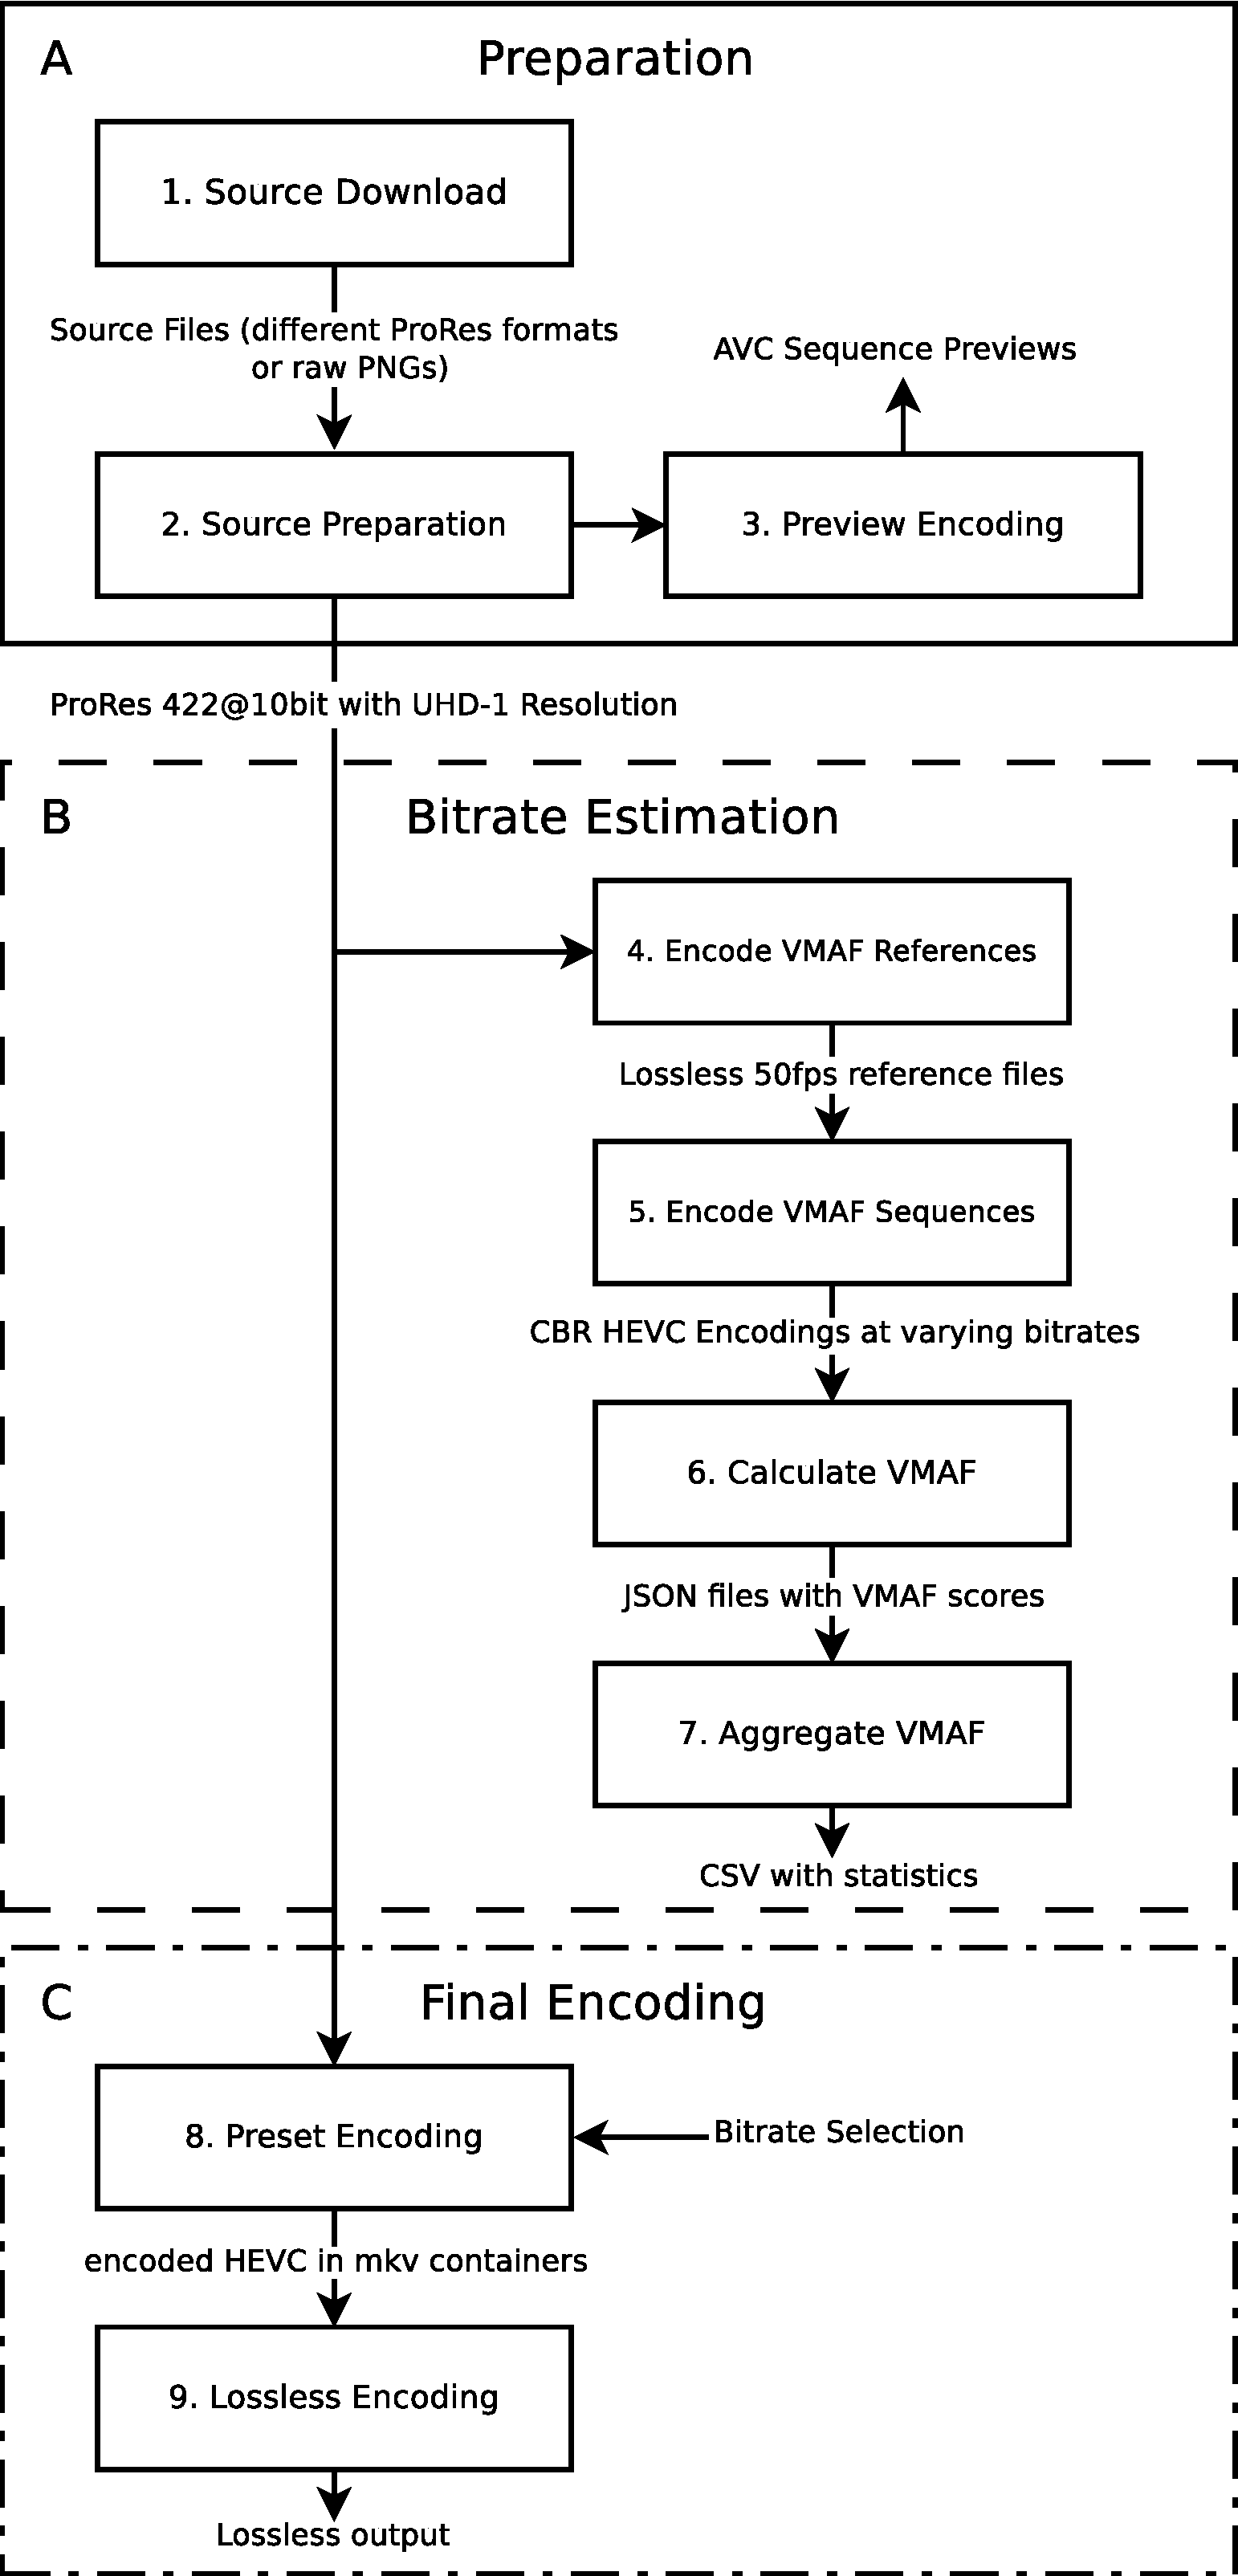
\includegraphics[width=1.28in]{automation}
	\end{figure}
\end{frame}

\begin{frame}
	\frametitle{Encoding Parameters}

	\begin{figure}[thb!]
		\centering
		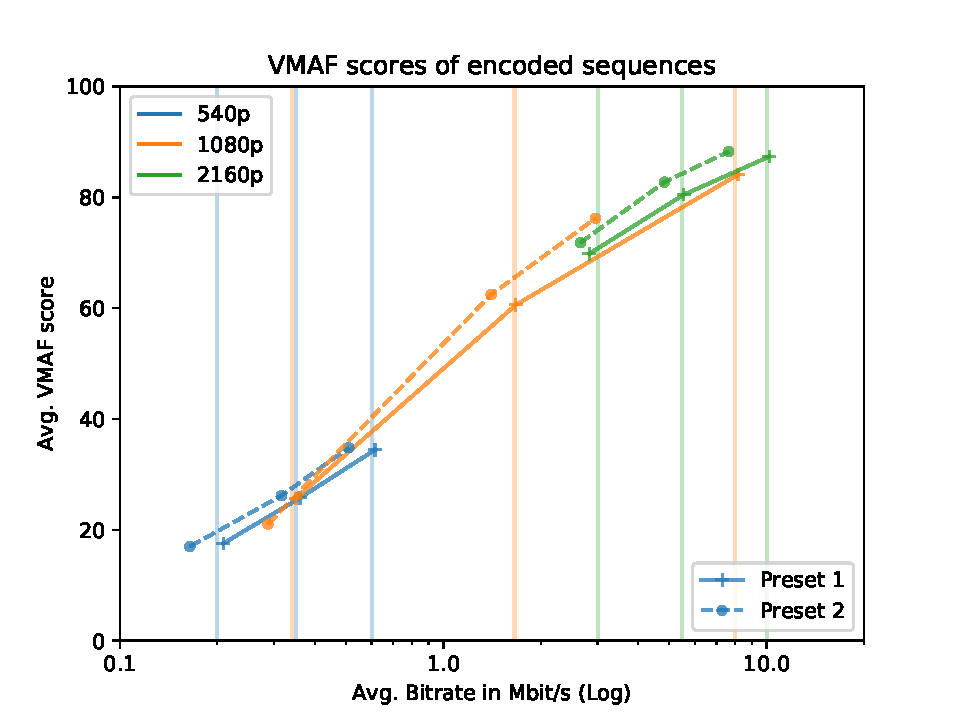
\includegraphics[width=2.8in]{vmaf_final}
	\end{figure}

	Average \textit{VMAF} scores of encoded videos for both presets.
\end{frame}
